
%(BEGIN_QUESTION)
% Copyright 2006, Tony R. Kuphaldt, released under the Creative Commons Attribution License (v 1.0)
% This means you may do almost anything with this work of mine, so long as you give me proper credit

I dette hydrauliske systemet blir en kraft på 25 N tilført det minste stempelet. Hvor stor kraft vil det store stempele generere? Regn også ut trykket i fluidet. 

$$\includegraphics[width=15.5cm]{i00150x01.eps}$$


\vskip 20pt \vbox{\hrule \hbox{\strut \vrule{} {\bf Suggestions for Socratic discussion} \vrule} \hrule}

\begin{itemize}
\item{} Identify which fundamental principles of science, technology, and/or math apply to each step of your solution to this problem.  In other words, be prepared to explain the reason(s) ``why'' for every step of your solution, rather than merely describing those steps.
\item{} Identify a practical application for a hydraulic system such as this.
\item{} Does the pressure/force/area equation hold true for all piston positions, or only with the pistons in mid-stroke as shown in the illustration?
\item{} Would it matter whether the fluid in this system was a liquid or a gas?  Explain in detail how the system's behavior would differ (or not differ) depending on the type of fluid used.
\item{} This mechanism seems to multiply the applied force.  How can it do so without violating the Law of Energy Conservation (energy out cannot exceed energy in)?
\item{} Demonstrate how to {\it estimate} numerical answers for this problem without using a calculator.
\end{itemize}

\underbar{file i00150}
%(END_QUESTION)





%(BEGIN_ANSWER)

Kraften = 100N
%(END_ANSWER)





%(BEGIN_NOTES)

Fluid pressure = 2500 Pa

\vskip 10pt

The 5 inch dimension is extraneous information, included for the purpose of challenging students to identify whether or not information is relevant to solving a particular problem.

\vskip 10pt

A common misconception among students is to think that Pascal's Principle {\it is} the mathematical relationship $P = {F \over A}$.  The correct definition of Pascal's Principle is the equal distribution of incremental pressure throughout a fluid system.






\vfil \eject

\noindent
{\bf Summary Quiz:}

Choose the best statement describing this hydraulic system:

$$\includegraphics[width=15.5cm]{i00150x02.eps}$$

\begin{itemize}
\item{} Force A and force B are equal; A moves further than B
\vskip 5pt 
\item{} Force A is greater than force B; A moves further than B 
\vskip 5pt 
\item{} Force B is greater than force A; A moves further than B 
\vskip 5pt 
\item{} Force A and force B are equal; B moves further than A
\vskip 5pt 
\item{} Force A is greater than force B; B moves further than A
\vskip 5pt 
\item{} Force B is greater than force A; B moves further than A 
\end{itemize}


%INDEX% Physics, fluids: pressure, force, and area
%INDEX% Physics, static fluids: Pascal's Principle

%(END_NOTES)


